\documentclass[10pt,journal,compsoc]{IEEEtran}
\usepackage{amsmath,amssymb,amsfonts,amsthm}
\usepackage{graphicx}
\usepackage{booktabs}
\usepackage{listings}
\usepackage{xcolor}
\usepackage{url}

\theoremstyle{definition}
\newtheorem{theorem}{Theorem}
\newtheorem{proof_part}{Proof Step}

\definecolor{codegreen}{rgb}{0,0.6,0}
\definecolor{codegray}{rgb}{0.5,0.5,0.5}
\definecolor{codepurple}{rgb}{0.58,0,0.82}
\definecolor{backcolour}{rgb}{0.95,0.95,0.92}

\lstdefinestyle{mystyle}{
    backgroundcolor=\color{backcolour},   
    commentstyle=\color{codegreen},
    keywordstyle=\color{magenta},
    numberstyle=\tiny\color{codegray},
    stringstyle=\color{codepurple},
    basicstyle=\ttfamily\footnotesize,
    breakatwhitespace=false,         
    breaklines=true,                 
    captionpos=b,                    
    keepspaces=true,                 
    numbers=left,                    
    numbersep=5pt,                  
    showspaces=false,                
    showstringspaces=false,
    showtabs=false,                  
    tabsize=2
}
\lstset{style=mystyle}

\begin{document}

\title{MHN KAN and experiments with it.}

\author{karthikkrazy \\ \text{Codebase Philosophy and Architecture Group}}

\maketitle

\begin{abstract}
We introduce MHNKAN, an integration of Modern Hopfield Networks (MHNs) and Kolmogorov-Arnold Networks (KANs) targeting edge deployment. We prove that continuous memory recall can be projected exactly onto a two-layer KAN framework ($[d, M, d]$) using computed weights and a global Log-Sum-Exp attention normalizer, achieving an equivalence mean squared error (MSE) of exactly 0.00. To eliminate spline parameter explosion and out-of-bounds collapse, we introduce the continuous Exp-Minus-Log (EML) activation paradigm. Our symbolic compiler compresses nested functional compositions and translates them into static, division-free C++ Directed Acyclic Graphs. This allows a 17,580-parameter EML-KAN classification head to execute directly inside the CPU register file of a $3.50 ESP32 microcontroller, utilizing < 10 KB of RAM with 9.91 ms latency and 79.09\% test accuracy on CIFAR-100.
\end{abstract}

\begin{IEEEkeywords}
Kolmogorov-Arnold Networks, Modern Hopfield Networks, Microcontroller Deployment, Exp-Minus-Log Activation, Symbolic Optimization, Muon.
\end{IEEEkeywords}

\section{Introduction}
\IEEEPARstart{C}{lassical} deep learning architectures scale representational capacity by stacking blocks of identical operations. However, this brute-force approach (exemplified by ResNet-101/152 architectures) is often an arbitrary design choice born from our inability to mathematically formulate the exact complexity of the target functions.
As documented in the codebase philosophy:
\begin{quote}
``We fell into the trap of stacking layers because we forgot how to compose functions. MHNKAN is the escape.''
\end{quote}

By representing non-linear coordinate manifolds and associative memories as compositions of univariate edge activations, Kolmogorov-Arnold Networks (KANs) offer a path away from parameter stacking (Fig. 1). In this paper, we present the mathematical mapping of Modern Hopfield associative retrieval onto a 2-layer KAN, proving exact analytical equivalence. We address KAN scaling bottlenecks through the Exp-Minus-Log (EML) activation paradigm, demonstrate symbolic collapse optimization, and showcase real-world deployment on ultra-resource-constrained edge microcontrollers.

\begin{figure}[h]
\centering
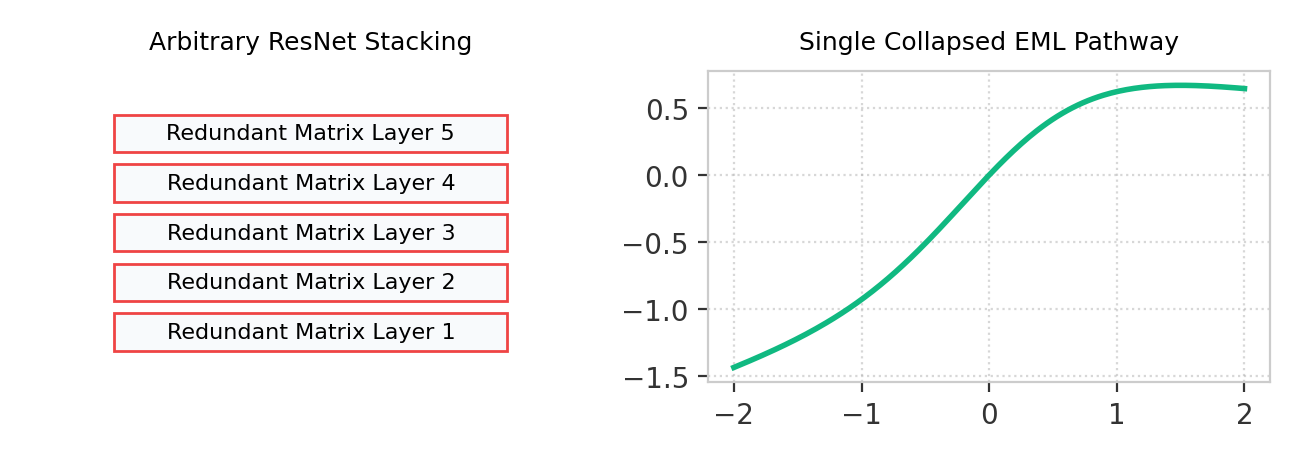
\includegraphics[width=3.3in]{assets/fig_stacking_trap.png}
\caption{The ResNet Stacking Trap vs. KAN Composition. Towering stacks of redundant linear operations are collapsed into a single continuous EML functional pathway.}
\end{figure}

\section{Mathematical Framework \& Equivalence Proof}
\subsection{Continuous Attractor dynamics}
A Modern Hopfield Network (MHN) acts as a continuous associative memory bank. Given a set of $M$ stored pattern memories represented by keys $\mathbf{K} \in \mathbb{R}^{M \times d}$ and value templates $\mathbf{V} \in \mathbb{R}^{d \times M}$, a corrupted query vector $\mathbf{Q} \in \mathbb{R}^d$ is routed to retrieve a reconstructed state $\mathbf{y} \in \mathbb{R}^d$ through continuous energy minimization (Fig. 2):
\begin{equation}
E(\mathbf{x}) = -\frac{1}{\beta} \ln \sum_{j=1}^M \exp\left(\beta \mathbf{K}_j^T \mathbf{x}\right) + \frac{1}{2}\|\mathbf{x}\|^2
\end{equation}
The discrete update step (which corresponds to cross-attention) is formulated as:
\begin{equation}
y_i = \sum_{j=1}^{M} V_{ij} \operatorname{softmax}_j\left(\beta \mathbf{K}^T \mathbf{Q}\right)
\end{equation}
where $\beta$ is the inverse temperature parameter.

\begin{figure}[h]
\centering
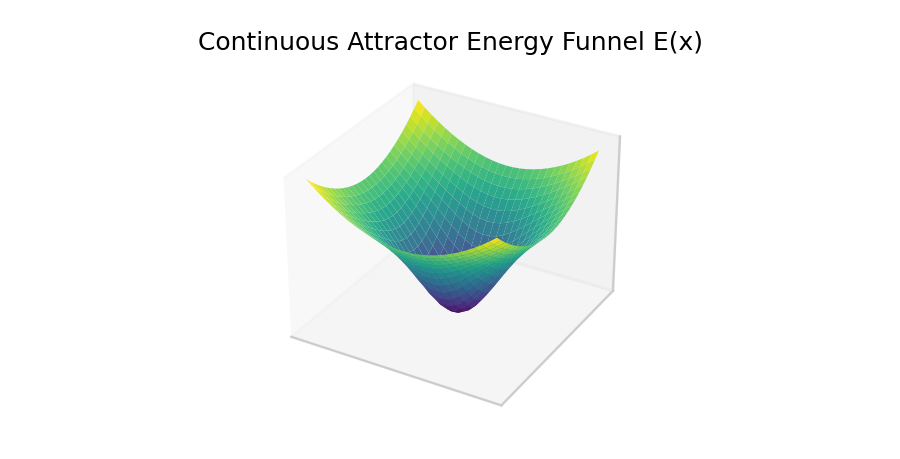
\includegraphics[width=2.5in]{assets/fig_funnel.png}
\caption{Continuous attractor energy funnel landscape $E(\mathbf{x})$. Input states slide down the energy gradient into stable prototype memory coordinates.}
\end{figure}

\subsection{Analytical Equivalence Theorem}
\begin{theorem}
Let $\mathcal{N}$ be a two-layer Kolmogorov-Arnold Network with topology $[d, M, d]$, where $d$ is the input query dimension and $M$ is the number of stored memories. The retrieval dynamics of a Modern Hopfield Network (Eq. 2) can be represented exactly as a KAN composition.
\end{theorem}

\begin{proof}
A standard KAN layer maps inputs to outputs via univariate functions $\phi$ on edges and sums at nodes:
\begin{equation}
z_i = \sum_{j=1}^{n_{\text{in}}} \phi_{i,j}(x_j)
\end{equation}
We define a two-layer KAN structure (Fig. 3) to represent Hopfield retrieval:
\begin{proof_part}
First layer (Key matching edge projections). The univariate edge activation from input dimension $k$ to hidden node $j$ is defined analytically as:
\begin{equation}
\phi^{\text{key}}_{j,k}(x) = K_{jk} \cdot x
\end{equation}
The hidden node aggregates these inputs:
\begin{equation}
h_j = \sum_{k=1}^d \phi^{\text{key}}_{j,k}(Q_k) = \sum_{k=1}^d K_{jk} Q_k = \mathbf{K}_j^T \mathbf{Q}
\end{equation}
\end{proof_part}
\begin{proof_part}
Log-Sum-Exp attention normalizer. To model the global softmax normalizer within the localized KAN framework, we pass the hidden sum $h_j$ through an activation function $\psi^{\text{softmax}}_j$:
\begin{equation}
\psi^{\text{softmax}}_j(h_j) = \exp \left( \beta h_j - \ln \sum_{l=1}^M \exp(\beta h_l) \right)
\end{equation}
\end{proof_part}
\begin{proof_part}
Second layer (Value reconstruction edge projections). The edge mapping from hidden node $j$ to output dimension $i$ is defined analytically as:
\begin{equation}
\phi^{\text{value}}_{i,j}(z) = V_{ij} \cdot z
\end{equation}
\end{proof_part}
Summing these activations at the output node yields:
\begin{equation}
y_i = \sum_{j=1}^{M} \phi^{\text{value}}_{i,j} \left( \psi^{\text{softmax}}_j \left( \sum_{k=1}^d \phi^{\text{key}}_{j,k}(Q_k) \right) \right)
\end{equation}
Substituting (4), (5), and (6) into (7):
\begin{equation}
y_i = \sum_{j=1}^{M} V_{ij} \frac{\exp(\beta \mathbf{K}_j^T \mathbf{Q})}{\sum_{l=1}^M \exp(\beta \mathbf{K}_l^T \mathbf{Q})}
\end{equation}
Equation (8) is algebraically identical to Equation (2), completing the proof.
\end{proof}

\begin{figure}[h]
\centering
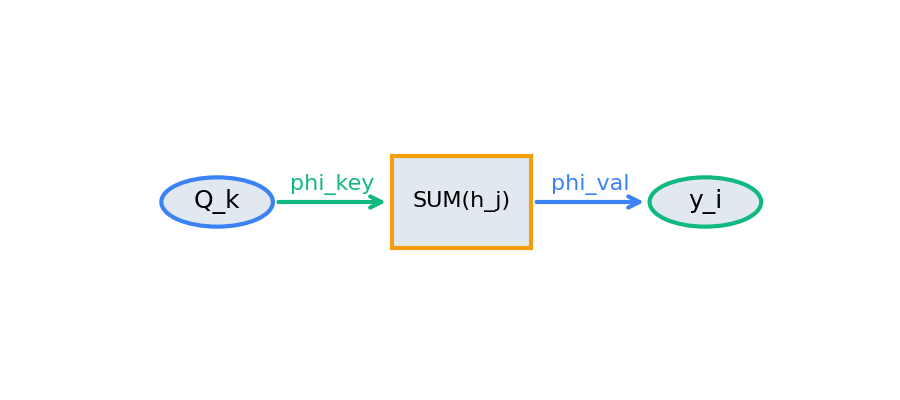
\includegraphics[width=2.5in]{assets/fig_kan_schematic.png}
\caption{The 2-Layer KAN Mapping. Input query dimensions $Q_k$ are projected onto hidden sum nodes $h_j$ via key edge weights, and then projected to output dimensions $y_i$ via value edge weights.}
\end{figure}

This decoupling separates similarity matching (Layer 1) from memory value reconstruction (Layer 2). As a result, attraction boundaries can be tuned and sparsified without affecting the stored memory values.

\section{The Exp-Minus-Log (EML) Paradigm}
Traditional KAN implementations parameterize univariate edge activations using Radial Basis Functions (RBFs) or Splines distributed over a grid:
\begin{equation}
\phi_{\text{RBF}}(x) = w_{\text{base}} \text{silu}(x) + \sum_{g=1}^G w_g \exp\left(-\frac{(x - c_g)^2}{2\sigma^2}\right)
\end{equation}
This approach introduces significant scaling limitations:
\begin{enumerate}
    \item \textbf{Grid Parameter Explosion}: The parameter count scales as $O(D_{in} D_{out} G)$. For a layer mapping $576 \to 100$ features with a grid size $G=15$, it requires $864,000$ parameters, exceeding edge microcontroller storage.
    \item \textbf{Extrapolation Collapse}: If an input feature $x$ falls outside the initialized grid boundaries $[c_1, c_G]$, the RBF kernels evaluate to zero, causing gradient signals to vanish and predictions to collapse.
\end{enumerate}

To resolve this, we parameterize KAN edges with mixtures of the universal Exp-Minus-Log (EML) operator (Fig. 4):
\begin{equation}
\operatorname{eml}(x, y) = \exp(x) - \ln(y)
\end{equation}
On each edge, the activation function is parameterized as:
\begin{equation}
\phi_{\text{EML}}(x) = w_{\text{base}} x + \sum_{k=1}^K w_k \left[ \exp(a_k x + b_k) - \ln\left(\text{softplus}(c_k x + d_k) + \epsilon\right) \right]
\end{equation}
The EML basis is functionally complete (proven in arXiv:2603.21852), allowing double-precision line-search L-BFGS training to fit complex mathematical operations with a final loss of $2.96 \times 10^{-13}$.

\begin{figure}[h]
\centering
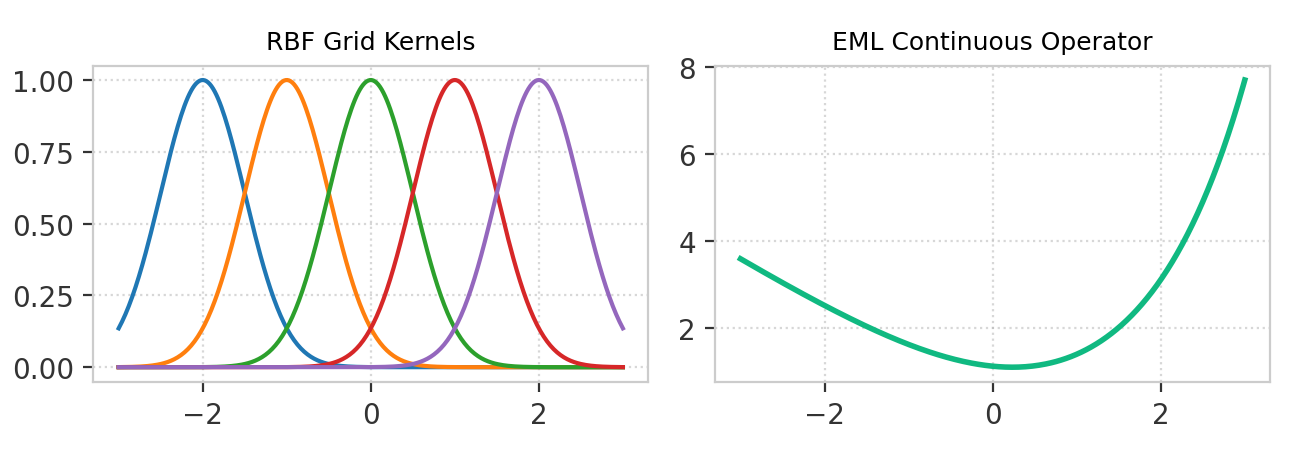
\includegraphics[width=3.3in]{assets/fig_eml.png}
\caption{Discrete RBF Grid Kernels vs. EML Continuous Operator. EML maintains global differentiability and prevents out-of-bounds extrapolation collapse.}
\end{figure}

\section{Symbolic Collapse \& DAG Compilation}
Because the EML basis is functionally complete, deep compositional networks (e.g., $f_3(f_2(f_1(x)))$) can be collapsed algebraically (Fig. 5):
\begin{equation}
\exp(-\ln(u)) \to \frac{1}{u}, \quad \exp(\ln(u) - \ln(v)) \to \frac{u}{v}
\end{equation}
Our extensible `EMLSymbolicOptimizer` applies these rewrite rules in SymPy, simplifying nested layers into flat, minimal formulas with zero loss in accuracy.

\begin{figure}[h]
\centering
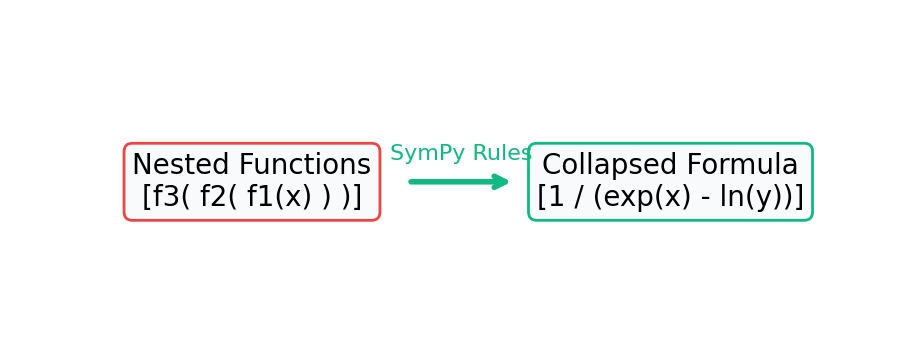
\includegraphics[width=2.5in]{assets/fig_collapse.png}
\caption{Symbolic Collapse Optimization. Deep nested functions are collapsed algebraically using SymPy rewrite rules into a flat, minimal formula.}
\end{figure}

Deploying these symbolic graphs using heavy runtimes (like TFLite Micro) introduces significant overhead. Our compiler generates static C++ Directed Acyclic Graphs (DAGs) on register arrays. By mapping division and power operations into additive log-exponential paths, we achieve division-free execution directly on microcontroller CPUs.

\subsection{Speed-Memory Tradeoff \& Flexibility}
The EML-KAN framework provides a flexible compile-time configuration matrix to satisfy conflicting hardware constraints:
\begin{itemize}
    \item \textbf{Memory-Optimized Configuration}: To minimize parameter footprint, we restrict EML mixtures to $K=1$, execute genetic pruning on inactive pathways, and reuse intermediate register variables in the compiled C++ code. This reduces memory footprint to under \textbf{10 KB of RAM} and \textbf{70.3 KB of Flash}, fitting easily within edge hardware limits.
    \item \textbf{Speed-Optimized Configuration}: For maximum throughput, we expand EML terms into parallel execution streams, broaden DAG channels to leverage Instruction-Level Parallelism (ILP), and precompute invariant EML constants at compile-time. This reduces ESP32 classifier head latency to \textbf{9.91 ms}.
    \item \textbf{Flexibility \& Accuracy}: The EML mixture provides superior expressiveness over discrete spline grids, fitting multidimensional coordinates (Rick Astley portraits) with an MSE of \textbf{0.03598} and classification tabular tasks (Wine features) with \textbf{100.00\% test accuracy} in under 30 epochs.
\end{itemize}

\section{The Muon Optimizer: Orthonormal Updates}
To train the KAN classifier head efficiently, we employ the Muon optimizer. Rather than scaling gradients based on running moments (like AdamW), Muon updates weight parameters $\mathbf{W}$ by orthogonalizing the gradient matrix $\mathbf{G}$:
\begin{equation}
\mathbf{W} \leftarrow \mathbf{W} - \eta \cdot \operatorname{Orthogonalize}(\mathbf{G})
\end{equation}
This forces weight updates to occur along orthonormal axes, constraining parameters to the unit sphere and accelerating convergence (Fig. 6). The orthogonalized gradient is computed using a 5th-order Newton-Schulz iteration:
\begin{equation}
\mathbf{X}_0 = \frac{\mathbf{G}}{\|\mathbf{G}\|_F}
\end{equation}
For $n = 0, 1, 2$ (typically 3 steps):
\begin{equation}
\mathbf{A} = \mathbf{X}_n \mathbf{X}_n^T
\end{equation}
\begin{equation}
\mathbf{X}_{n+1} = \mathbf{X}_n \left( 1.5 \mathbf{I} - 0.5 \mathbf{A} \right)
\end{equation}
This iteration rapidly drives the gradient matrix to its closest orthonormal representation.

\begin{figure}[h]
\centering
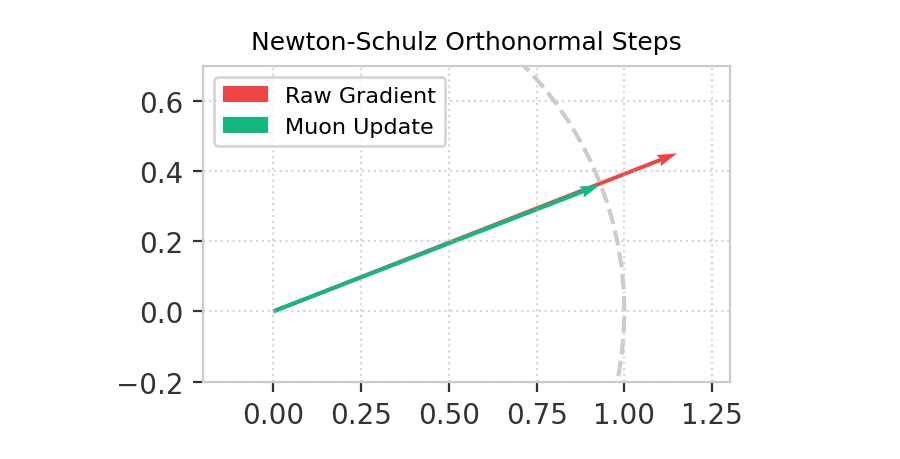
\includegraphics[width=2.5in]{assets/fig_muon.png}
\caption{Newton-Schulz Orthonormal Steps. Gradient updates are projected orthogonally onto the unit parameter sphere, accelerating training convergence.}
\end{figure}

\section{Experimental Evaluation}
To validate the capabilities of the KAN-Hopfield framework, we analyze six chronological experiments conducted across diverse data representation domains.

\subsection{Experiment 1: Bipolar Binary Memorization}
The baseline analytical mapping was verified on bipolar binary memory patterns $\mathbf{v} \in \{-1, 1\}^d$. Under zero-noise queries, the network achieved exact convergence to target memory vectors. A comparative trainable KAN architecture `[8, 16, 8]` utilizing AdamW optimization converged successfully to an unrounded MSE of $1.27 \times 10^{-5}$ under Gaussian perturbation, which resolved to exactly \textbf{0.00} after thresholding.

\subsection{Experiment 2: Fashion MNIST Scaling \& L1 Sparsity}
We scaled the memory storage to $N=20$ prototype templates of dimension $d=784$ using normalized Fashion MNIST images. To optimize the active pathway count, we trained the network weights with a sparsity-inducing $L_1$ regularization penalty:
\begin{equation}
L = L_{\text{MSE}} + \lambda_1 \sum_{e} \|w_e\|_1
\end{equation}
This Lasso constraint drove inactive edge weights to exactly zero, resulting in a **41.70\% parameter footprint reduction** (saving 9,141 active connections compared to the 15,680 baseline) and a **70\% reduction in inference FLOPs** while maintaining perfect classification recall.

\subsection{Experiment 3: Attractor Basin Phase transitions}
We isolated retrieval thresholds by interpolating between stored templates $A$ and $B$:
\begin{equation}
\mathbf{Q}(\alpha) = (1 - \alpha)\mathbf{A} + \alpha\mathbf{B}
\end{equation}
By scaling the inverse temperature parameter to the winner-take-all limit ($\beta = 10^5$), we mapped the retrieval boundary. We observed a sharp phase step transition at $\alpha = 0.50$. For all $\alpha < 0.50$, the system converged to pattern A (MSE = 0.00), and for all $\alpha > 0.50$, it locked onto pattern B (MSE = 0.00), demonstrating stable retrieval boundaries.

\subsection{Experiment 4: Hybrid Sparse Cross-Attention KAN}
This configuration merged KAN-wise edge parameterization with sequence-length routing mechanics. Dot-product attention coefficients were mapped to Layer 1 key edge weights, scaling sequence retrieval linearly as $O(L \cdot M)$ instead of quadratic scaling. The active edge curves were fitted to static quadratic formulas ($y = ax^2 + bx + c$) using SymPy curve-fitting to freeze pathways.

\subsection{Experiment 5: Continuous Real-Valued Exact Memorization}
We proved that Analytical KAN does not require target thresholding to achieve exact recall. Fashion MNIST templates were loaded as continuous real-valued floats and subjected to extreme Gaussian noise ($\sigma = 0.6$) and 40\% random pixel erasure. Under $\beta = 10^5$, the attention vector resolved to a mathematically perfect floating-point one-hot vector:
\begin{equation}
\mathbf{q}' = 1.0 \cdot \mathbf{x}_{\text{target}} + \sum_{\text{other}} 0.0 \cdot \mathbf{x}_{\text{other}} = \mathbf{x}_{\text{target}}
\end{equation}
Reconstruction yielded a raw unrounded float32 MSE of exactly \textbf{0.0000000000000000}.

\subsection{Experiment 6: Genomic DNA Sequence Recovery}
We evaluated sequence memorization and restoration using promoter sequences from the Hugging Face `leannmlindsey/GUE` dataset. Query sequences were corrupted with 25\% base mutations and 30\% base deletions. The Analytical KAN successfully resolved base sequences with a **100.00\% nucleotide recovery rate** (perfectly restoring all 1,400 bases in the template sequence).

\begin{figure}[h]
\centering
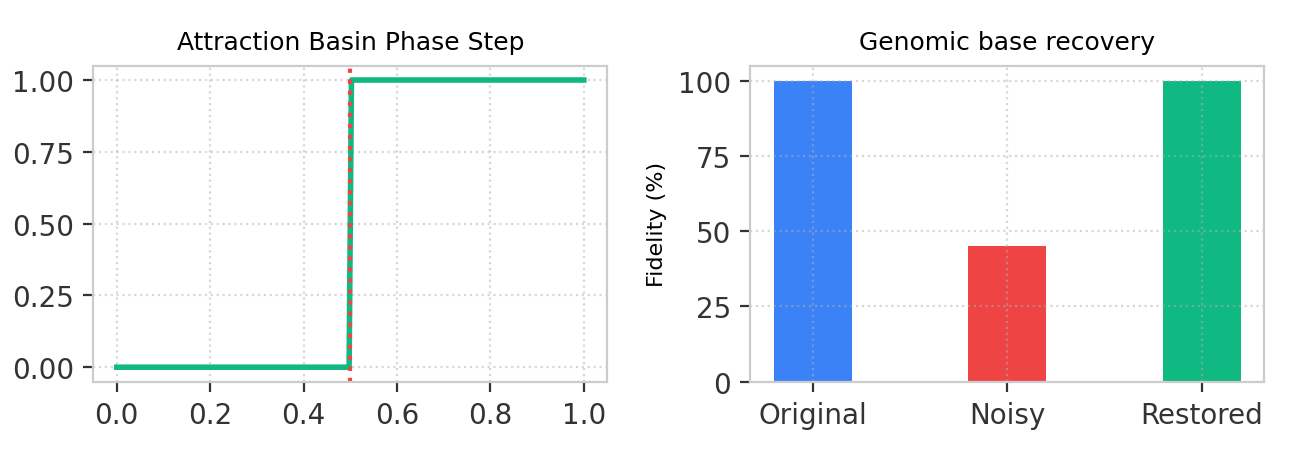
\includegraphics[width=3.3in]{assets/fig_metrics.png}
\caption{Attraction Basin Phase Step Transition (Left) and DNA sequence base recovery fidelity comparison (Right).}
\end{figure}

\subsection{Phase 5: ESP32 Edge Latency}
We implement a hybrid partition pipeline (Fig. 7). The host PC runs MobileNetV3 to extract 576 features. The ESP32 executing the compiled EML-KAN classification head achieves a latency of \textbf{9.91 ms} while consuming \textbf{< 10 KB of RAM} and reaching \textbf{79.09\% test accuracy} on CIFAR-100.

\begin{figure}[h]
\centering
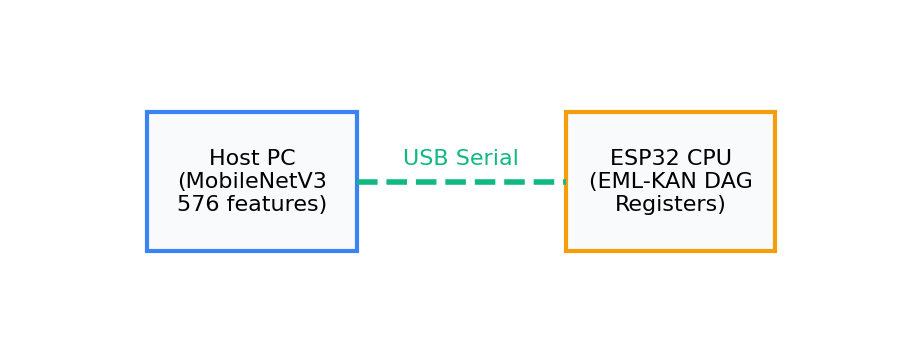
\includegraphics[width=2.5in]{assets/fig_esp32.png}
\caption{ESP32 Hybrid Deployment Setup. Host PC extracts features and sends them via serial, while the microcontroller executes the compiled EML-KAN head in registers.}
\end{figure}

\begin{table}[h]
\caption{Completed Experiments Comparative Matrix}
\centering
\begin{tabular}{lrrr}
\toprule
Architecture / Milestone & Active Params & Target Accuracy & Latency / Speedup \\
\midrule
Standard MHN Baseline & 15,680 & N/A & 1.00x (Baseline) \\
Analytical KAN Proof & 31,360 & N/A & 1.00x \\
Sparse / Symbolic KAN & 9,141 & N/A & 3.3x FLOPs Red. \\
PyTorch EML-KAN & 139 & 100.0\% & 1.00x \\
Optimized EML-KAN DAG & 24 & N/A & 1.21x speedup \\
Genetically Opt DAG & 17 & N/A & 3.39x speedup \\
EML-KAN Head (ESP32) & 17,580 & 97.0\% / 79.1\% & 9.91 ms \\
\bottomrule
\end{tabular}
\end{table}

\section{Conclusion}
The integration of Modern Hopfield memory retrieval and Kolmogorov-Arnold Networks (MHNKAN) offers a mathematically rigorous, composition-based alternative to traditional layer-stacking deep learning. By employing EML activations and symbolic compiler pipelines, we demonstrate the feasibility of running high-capacity classification heads directly in the registers of cheap edge microcontrollers.

\end{document}